\documentclass{standalone}
\usepackage{tikz}
\usetikzlibrary{patterns, positioning}


\begin{document}
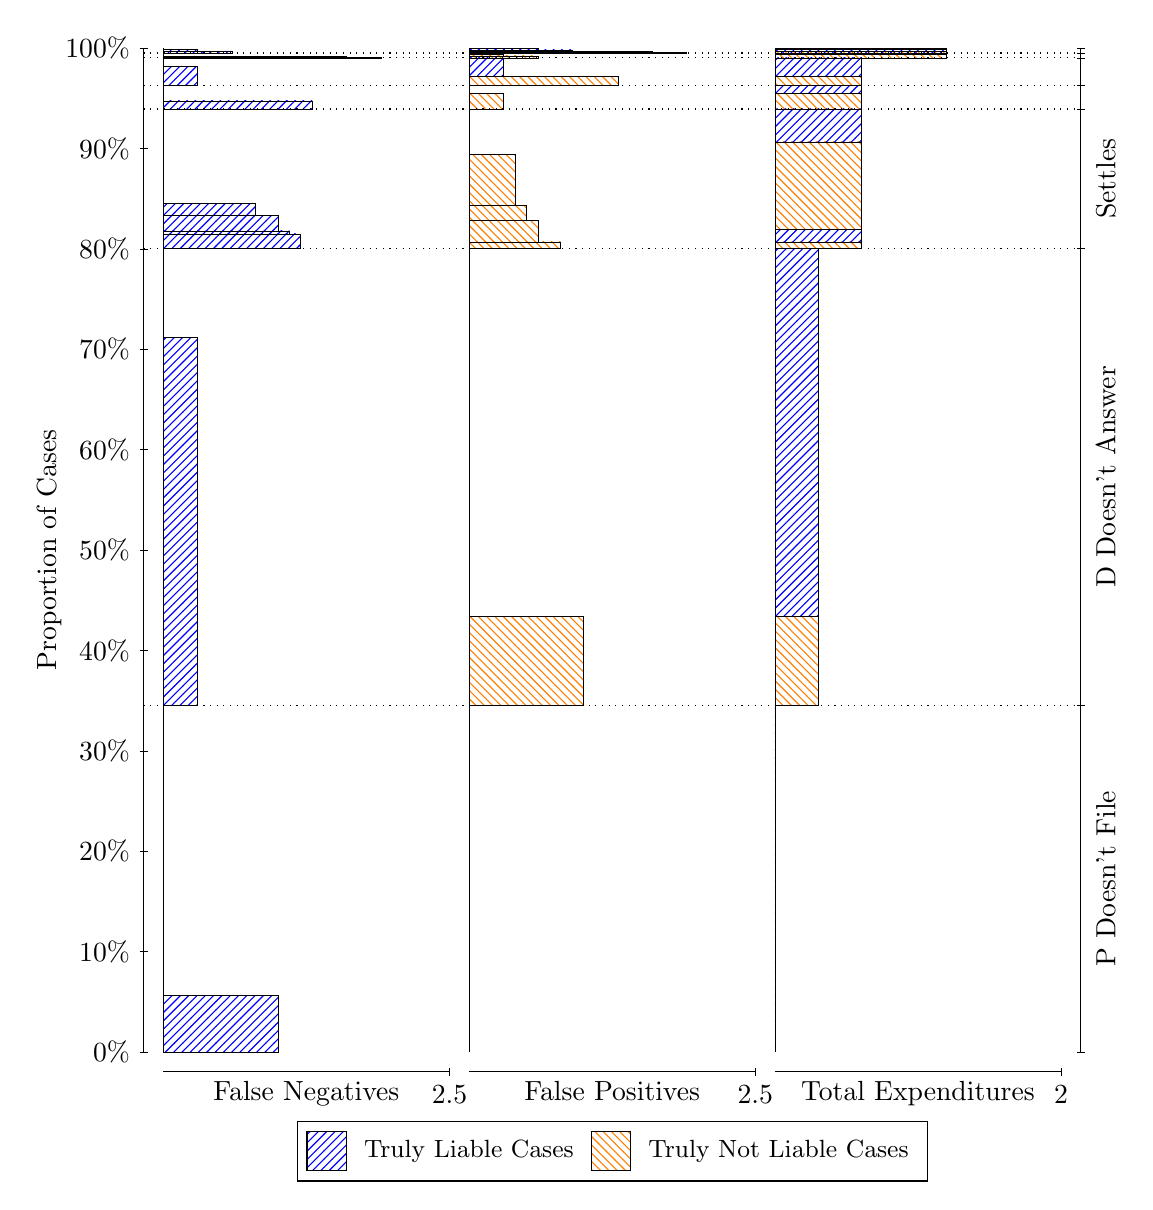
\begin{tikzpicture}
\draw[black, very thin] (1.5,1.75) -- (1.5,14.5);
\node[rotate=90, text=black, anchor=center] at (0.3, 8.125) {Proportion of Cases};
\draw[black, very thin] (1.45,1.75) -- (1.55,1.75);
\node[text=black, anchor=east] at (1.45, 1.75) {0\%};
\draw[black, very thin] (1.45,3.025) -- (1.55,3.025);
\node[text=black, anchor=east] at (1.45, 3.025) {10\%};
\draw[black, very thin] (1.45,4.3) -- (1.55,4.3);
\node[text=black, anchor=east] at (1.45, 4.3) {20\%};
\draw[black, very thin] (1.45,5.575) -- (1.55,5.575);
\node[text=black, anchor=east] at (1.45, 5.575) {30\%};
\draw[black, very thin] (1.45,6.85) -- (1.55,6.85);
\node[text=black, anchor=east] at (1.45, 6.85) {40\%};
\draw[black, very thin] (1.45,8.125) -- (1.55,8.125);
\node[text=black, anchor=east] at (1.45, 8.125) {50\%};
\draw[black, very thin] (1.45,9.4) -- (1.55,9.4);
\node[text=black, anchor=east] at (1.45, 9.4) {60\%};
\draw[black, very thin] (1.45,10.675) -- (1.55,10.675);
\node[text=black, anchor=east] at (1.45, 10.675) {70\%};
\draw[black, very thin] (1.45,11.95) -- (1.55,11.95);
\node[text=black, anchor=east] at (1.45, 11.95) {80\%};
\draw[black, very thin] (1.45,13.225) -- (1.55,13.225);
\node[text=black, anchor=east] at (1.45, 13.225) {90\%};
\draw[black, very thin] (1.45,14.5) -- (1.55,14.5);
\node[text=black, anchor=east] at (1.45, 14.5) {100\%};

\draw[black, very thin] (13.4,1.75) -- (13.4,14.5);
\draw[black, very thin] (13.35,1.75) -- (13.45,1.75);
\node[anchor=west] at (13.35, 1.75) {};
\draw[black, very thin] (13.35,6.1534) -- (13.45,6.1534);
\node[anchor=west] at (13.35, 6.1534) {};
\draw[black, very thin] (13.35,11.954) -- (13.45,11.954);
\node[anchor=west] at (13.35, 11.954) {};
\draw[black, very thin] (13.35,13.726) -- (13.45,13.726);
\node[anchor=west] at (13.35, 13.726) {};
\draw[black, very thin] (13.35,14.026) -- (13.45,14.026);
\node[anchor=west] at (13.35, 14.026) {};
\draw[black, very thin] (13.35,14.376) -- (13.45,14.376);
\node[anchor=west] at (13.35, 14.376) {};
\draw[black, very thin] (13.35,14.437) -- (13.45,14.437);
\node[anchor=west] at (13.35, 14.437) {};
\draw[black, very thin] (13.35,14.5) -- (13.45,14.5);
\node[anchor=west] at (13.35, 14.5) {};

\draw[black, very thin, pattern color=blue, pattern=north east lines] (1.75,1.75) rectangle (3.2033,2.4682);
\draw[black, very thin, pattern color=orange, pattern=north west lines] (1.75,2.4682) rectangle (1.75,6.1534);
\draw[black, very thin, pattern color=blue, pattern=north east lines] (1.75,6.1534) rectangle (2.186,10.83);
\draw[black, very thin, pattern color=orange, pattern=north west lines] (1.75,10.83) rectangle (1.75,11.954);
\draw[black, very thin, pattern color=blue, pattern=north east lines] (1.75,11.954) rectangle (3.494,12.139);
\draw[black, very thin, pattern color=blue, pattern=north east lines] (1.75,12.139) rectangle (3.3487,12.178);
\draw[black, very thin, pattern color=blue, pattern=north east lines] (1.75,12.178) rectangle (3.2033,12.372);
\draw[black, very thin, pattern color=blue, pattern=north east lines] (1.75,12.372) rectangle (2.9127,12.527);
\draw[black, very thin, pattern color=orange, pattern=north west lines] (1.75,12.527) rectangle (1.75,13.726);
\draw[black, very thin, pattern color=blue, pattern=north east lines] (1.75,13.726) rectangle (3.6393,13.83);
\draw[black, very thin, pattern color=orange, pattern=north west lines] (1.75,13.83) rectangle (1.75,14.026);
\draw[black, very thin, pattern color=blue, pattern=north east lines] (1.75,14.026) rectangle (2.186,14.266);
\draw[black, very thin, pattern color=orange, pattern=north west lines] (1.75,14.266) rectangle (1.75,14.376);
\draw[black, very thin, pattern color=blue, pattern=north east lines] (1.75,14.376) rectangle (4.5113,14.381);
\draw[black, very thin, pattern color=blue, pattern=north east lines] (1.75,14.381) rectangle (4.0753,14.397);
\draw[black, very thin, pattern color=orange, pattern=north west lines] (1.75,14.397) rectangle (1.75,14.437);
\draw[black, very thin, pattern color=blue, pattern=north east lines] (1.75,14.437) rectangle (2.622,14.462);
\draw[black, very thin, pattern color=blue, pattern=north east lines] (1.75,14.462) rectangle (2.186,14.479);
\draw[black, very thin, pattern color=orange, pattern=north west lines] (1.75,14.479) rectangle (1.75,14.5);
\draw[black, very thin, pattern color=orange, pattern=north west lines] (5.6333,1.75) rectangle (5.6333,5.4351);
\draw[black, very thin, pattern color=blue, pattern=north east lines] (5.6333,5.4351) rectangle (5.6333,6.1534);
\draw[black, very thin, pattern color=orange, pattern=north west lines] (5.6333,6.1534) rectangle (7.0867,7.2782);
\draw[black, very thin, pattern color=blue, pattern=north east lines] (5.6333,7.2782) rectangle (5.6333,11.954);
\draw[black, very thin, pattern color=orange, pattern=north west lines] (5.6333,11.954) rectangle (6.796,12.037);
\draw[black, very thin, pattern color=orange, pattern=north west lines] (5.6333,12.037) rectangle (6.5053,12.311);
\draw[black, very thin, pattern color=orange, pattern=north west lines] (5.6333,12.311) rectangle (6.36,12.497);
\draw[black, very thin, pattern color=orange, pattern=north west lines] (5.6333,12.497) rectangle (6.2147,13.153);
\draw[black, very thin, pattern color=blue, pattern=north east lines] (5.6333,13.153) rectangle (5.6333,13.726);
\draw[black, very thin, pattern color=orange, pattern=north west lines] (5.6333,13.726) rectangle (6.0693,13.921);
\draw[black, very thin, pattern color=blue, pattern=north east lines] (5.6333,13.921) rectangle (5.6333,14.026);
\draw[black, very thin, pattern color=orange, pattern=north west lines] (5.6333,14.026) rectangle (7.5227,14.136);
\draw[black, very thin, pattern color=blue, pattern=north east lines] (5.6333,14.136) rectangle (6.0693,14.376);
\draw[black, very thin, pattern color=orange, pattern=north west lines] (5.6333,14.376) rectangle (6.5053,14.4);
\draw[black, very thin, pattern color=orange, pattern=north west lines] (5.6333,14.4) rectangle (6.0693,14.416);
\draw[black, very thin, pattern color=blue, pattern=north east lines] (5.6333,14.416) rectangle (5.6333,14.437);
\draw[black, very thin, pattern color=orange, pattern=north west lines] (5.6333,14.437) rectangle (8.3947,14.442);
\draw[black, very thin, pattern color=orange, pattern=north west lines] (5.6333,14.442) rectangle (7.9587,14.458);
\draw[black, very thin, pattern color=blue, pattern=north east lines] (5.6333,14.458) rectangle (6.9413,14.475);
\draw[black, very thin, pattern color=blue, pattern=north east lines] (5.6333,14.475) rectangle (6.5053,14.5);
\draw[black, very thin, pattern color=orange, pattern=north west lines] (9.5167,1.75) rectangle (9.5167,5.4351);
\draw[black, very thin, pattern color=blue, pattern=north east lines] (9.5167,5.4351) rectangle (9.5167,6.1534);
\draw[black, very thin, pattern color=orange, pattern=north west lines] (9.5167,6.1534) rectangle (10.062,7.2782);
\draw[black, very thin, pattern color=blue, pattern=north east lines] (9.5167,7.2782) rectangle (10.062,11.954);
\draw[black, very thin, pattern color=orange, pattern=north west lines] (9.5167,11.954) rectangle (10.607,12.037);
\draw[black, very thin, pattern color=blue, pattern=north east lines] (9.5167,12.037) rectangle (10.607,12.192);
\draw[black, very thin, pattern color=orange, pattern=north west lines] (9.5167,12.192) rectangle (10.607,13.308);
\draw[black, very thin, pattern color=blue, pattern=north east lines] (9.5167,13.308) rectangle (10.607,13.726);
\draw[black, very thin, pattern color=orange, pattern=north west lines] (9.5167,13.726) rectangle (10.607,13.921);
\draw[black, very thin, pattern color=blue, pattern=north east lines] (9.5167,13.921) rectangle (10.607,14.026);
\draw[black, very thin, pattern color=orange, pattern=north west lines] (9.5167,14.026) rectangle (10.607,14.136);
\draw[black, very thin, pattern color=blue, pattern=north east lines] (9.5167,14.136) rectangle (10.607,14.376);
\draw[black, very thin, pattern color=orange, pattern=north west lines] (9.5167,14.376) rectangle (11.697,14.416);
\draw[black, very thin, pattern color=blue, pattern=north east lines] (9.5167,14.416) rectangle (11.697,14.437);
\draw[black, very thin, pattern color=orange, pattern=north west lines] (9.5167,14.437) rectangle (11.697,14.453);
\draw[black, very thin, pattern color=blue, pattern=north east lines] (9.5167,14.453) rectangle (11.697,14.478);
\draw[black, very thin, pattern color=orange, pattern=north west lines] (9.5167,14.478) rectangle (11.697,14.483);
\draw[black, very thin, pattern color=blue, pattern=north east lines] (9.5167,14.483) rectangle (11.697,14.5);
\draw[black, dotted] (1.5,6.1534) -- (13.4,6.1534);
\draw[black, dotted] (1.5,11.954) -- (13.4,11.954);
\draw[black, dotted] (1.5,13.726) -- (13.4,13.726);
\draw[black, dotted] (1.5,14.026) -- (13.4,14.026);
\draw[black, dotted] (1.5,14.376) -- (13.4,14.376);
\draw[black, dotted] (1.5,14.437) -- (13.4,14.437);
\draw[black, very thin] (1.75,1.5) -- (5.3833,1.5);
\node[text=black, anchor=north] at (3.5667, 1.5) {False Negatives};
\draw[black, very thin] (5.3833,1.45) -- (5.3833,1.55);
\node[text=black, anchor=north] at (5.3833, 1.45) {2.5};

\draw[black, very thin] (5.6333,1.5) -- (9.2667,1.5);
\node[text=black, anchor=north] at (7.45, 1.5) {False Positives};
\draw[black, very thin] (9.2667,1.45) -- (9.2667,1.55);
\node[text=black, anchor=north] at (9.2667, 1.45) {2.5};

\draw[black, very thin] (9.5167,1.5) -- (13.15,1.5);
\node[text=black, anchor=north] at (11.333, 1.5) {Total Expenditures};
\draw[black, very thin] (13.15,1.45) -- (13.15,1.55);
\node[text=black, anchor=north] at (13.15, 1.45) {2};

\node[text=black, centered, rotate=90] at (13.72, 3.9517) {P Doesn't File};
\node[text=black, centered, rotate=90] at (13.72, 9.0538) {D Doesn't Answer};
\node[text=black, centered, rotate=90] at (13.72, 12.84) {Settles};





\draw (7.449999999999999,1.5) node[draw=none] (baseCoordinate) {};
\begin{scope}[align=center]
        \matrix[scale=0.5, draw=black, below=0.5cm of baseCoordinate, nodes={draw}, column sep=0.1cm]{
            \node[rectangle, draw, minimum width=0.5cm, minimum height=0.5cm, pattern color=blue, pattern=north east lines] {}; &
            \node[draw=none, font=\small, text=black] (B) {Truly Liable Cases}; &
            \node[rectangle, draw, minimum width=0.5cm, minimum height=0.5cm, pattern color=orange, pattern=north west lines] {}; &
            \node[draw=none, font=\small, text=black] (B) {Truly Not Liable Cases}; \\
            };
\end{scope}

\end{tikzpicture}
\end{document}